% Book 4, Year 2, chapter 26 -- Flows and matchings.
% Provenance (never printed): sources/book4/BRIEFS.md, chapter 26.
\chapter{Flows and Matchings}\label{ch:b2:flows-and-matchings}

On the day of a match, buses leave the town's Bus Depot for the Football Ground. Every road can carry only so many buses
an hour; the rule used in this chapter is that a road with a speed limit of $v$ km/h carries $v - 10$ buses an hour in
each direction it is open. How many buses an hour can reach the ground? A program answers in a few lines:

\omcode{code/bachelor-2/26-flows-and-matchings/listings/town_flow.py}{5}{16}{The largest number of buses an hour from the
depot (place 16) to the ground (place 15), and the roads that limit it}\label{lst:b2:flows-and-matchings:town}

\omoutput{code/bachelor-2/26-flows-and-matchings/outputs/town_flow.txt}{Five routes found one after the other, 120 buses
an hour in all, and four roads that carry exactly 120 between them.}\label{out:b2:flows-and-matchings:town}

Two numbers agree in that output: the 120 buses an hour sent, and the 120 that four roads can carry. The second is a
proof that nobody can do better, since every bus from the depot to the ground has to use one of those four roads. This
chapter proves that such a pair of numbers always exists, gives an algorithm that finds both in polynomial time, and
then uses it for problems that do not look like traffic at all: pairing readers with reading slots, finding routes with
no road in common, and choosing which projects to run.

\begin{recall}
The Year 1 volume: directed graphs and their adjacency lists; breadth-first search, which finds the paths with fewest
edges from a vertex; bipartite graphs, whose vertices split into two sides with every edge going from one side to the
other; the \omterm{def:b2:flows-and-matchings:cut}{cut} of a graph, a split of its vertices into two parts, used there for minimum spanning trees.
\end{recall}

\section{Flow networks and cuts}\label{sec:b2:flows-and-matchings:networks}

\begin{definition}[Flow network]\label{def:b2:flows-and-matchings:network}
A \emph{flow network}\index{flow network} is a directed graph $G = (V, E)$ with two distinct vertices, the
\emph{source}\index{source (flow network)} $s$ and the \emph{sink}\index{sink (flow network)} $t$, and a
\emph{capacity}\index{capacity (flow network)} $c(u, v) \geq 0$ for each edge $(u, v)$. We set $c(u, v) = 0$ when $(u, v)$
is not an edge.
\end{definition}

\begin{definition}[Flow, value]\label{def:b2:flows-and-matchings:flow}
A \emph{flow}\index{flow (network)} is a function $f$ on the edges with
\begin{itemize}
\item \emph{capacity}: $0 \leq f(u, v) \leq c(u, v)$ for every edge;
\item \emph{conservation}: for every vertex $w \neq s, t$, what enters equals what leaves,
$\sum_{u} f(u, w) = \sum_{v} f(w, v)$.
\end{itemize}
Its \emph{value}\index{value of a flow} is what leaves the \omterm{def:b2:flows-and-matchings:network}{source}, less what enters it:
$|f| = \sum_{v} f(s, v) - \sum_{u} f(u, s)$. A \emph{maximum flow} is a flow of largest value.
\end{definition}

In \cref{out:b2:flows-and-matchings:town} the vertices are the town's places, the edges its roads in each direction
they are open, the capacities buses an hour, and the \omterm{def:b2:flows-and-matchings:flow}{flow} the number of buses an hour planned on each road. Conservation
says that buses neither appear nor vanish at a junction. The smaller network below serves for the hand computations of
the chapter.

\omoutput{code/bachelor-2/26-flows-and-matchings/outputs/flow.txt}{A maximum \omterm{def:b2:flows-and-matchings:flow}{flow} of a network with six vertices, found
in three augmentations, and the \omterm{def:b2:flows-and-matchings:cut}{cut} that proves it maximum.}\label{out:b2:flows-and-matchings:flow}

\begin{omfigure}
\begin{tikzpicture}[x=13mm, y=12mm, v/.style={circle, draw, thick, minimum size=7mm, inner sep=0pt},
  e/.style={->, >=Stealth, thick}, lab/.style={font=\small, fill=white, inner sep=1pt}]
\node[v] (s) at (0, 0) {$s$};
\node[v] (a) at (2, 1.2) {$a$};
\node[v] (d) at (4.4, 1.2) {$d$};
\node[v] (b) at (2, -1.2) {$b$};
\node[v] (c) at (4.4, -1.2) {$c$};
\node[v] (t) at (6.4, 0) {$t$};
\draw[e, red!70!black] (s) -- node[lab] {8/8} (a);
\draw[e] (s) -- node[lab] {4/6} (b);
\draw[e] (a) -- node[lab, pos=0.68] {3/7} (c);
\draw[e, red!70!black] (a) -- node[lab, above=1pt, pos=0.25] {5/5} (d);
\draw[e] (b) -- node[lab] {4/6} (c);
\draw[e, red!70!black] (c) -- node[lab, pos=0.3] {7/7} (t);
\draw[e] (d) -- node[lab] {5/9} (t);
\draw[dashed, very thick, blue!60!black] (3.2, 2) -- (3.2, 0.4) -- (5.4, -0.3) -- (5.4, -2)
  node[below, font=\small] {cut};
\node[font=\small, blue!60!black] at (0.6, -1.9) {$S = \{s, a, b, c\}$};
\node[font=\small, blue!60!black] at (6.4, 1.5) {$T = \{d, t\}$};
\end{tikzpicture}
\par\smallskip{\small The network of \cref{out:b2:flows-and-matchings:flow} with its maximum \omterm{def:b2:flows-and-matchings:flow}{flow}, each edge labelled
\omterm{def:b2:flows-and-matchings:flow}{flow}/capacity; saturated edges are red. The dashed line is the minimum \omterm{def:b2:flows-and-matchings:cut}{cut}: the edges from $S$ to $T$ are $(a, d)$ and
$(c, t)$, both saturated, of total capacity $5 + 7 = 12$, the \omterm{def:b2:flows-and-matchings:flow}{value} of the \omterm{def:b2:flows-and-matchings:flow}{flow}.}
\end{omfigure}

\begin{definition}[Cut of a flow network, capacity]\label{def:b2:flows-and-matchings:cut}
A \emph{cut}\index{cut (flow network)} of a \omterm{def:b2:flows-and-matchings:network}{flow network} is a partition of $V$ into two sets $S$ and $T = V \setminus S$
with $s \in S$ and $t \in T$. Its \emph{capacity}\index{capacity of a cut} is $c(S, T) = \sum_{u \in S,\, v \in T} c(u,
v)$, the capacities of the edges from $S$ to $T$ only. The \emph{net \omterm{def:b2:flows-and-matchings:flow}{flow}} across it is $f(S, T) = \sum_{u \in S,\, v \in
T} f(u, v) - \sum_{u \in T,\, v \in S} f(u, v)$.
\end{definition}

The \omterm{def:b2:flows-and-matchings:cut}{cut} of a \omterm{def:b2:flows-and-matchings:network}{flow network} is the \omterm{def:b2:flows-and-matchings:cut}{cut} of a graph of the Year 1 volume with a side chosen for $s$ and one for $t$, and it
counts only the edges that go forwards, from $S$ to $T$.

\begin{proposition}[Flow across a cut]\label{prop:b2:flows-and-matchings:flow-across-cut}
For every \omterm{def:b2:flows-and-matchings:flow}{flow} $f$ and every \omterm{def:b2:flows-and-matchings:cut}{cut} $(S, T)$, $f(S, T) = |f|$.
\end{proposition}

\begin{proof}
\Cref{exo:b2:flows-and-matchings:8}: sum the conservation equations over the vertices of $S$ other than $s$.
\end{proof}

\begin{corollary}[Weak duality]\label{cor:b2:flows-and-matchings:weak-duality}
For every \omterm{def:b2:flows-and-matchings:flow}{flow} $f$ and every \omterm{def:b2:flows-and-matchings:cut}{cut} $(S, T)$, $|f| \leq c(S, T)$. So if $|f| = c(S, T)$, the \omterm{def:b2:flows-and-matchings:flow}{flow} is maximum and the \omterm{def:b2:flows-and-matchings:cut}{cut} is
of minimum capacity.
\end{corollary}

\begin{proof}
$|f| = f(S, T) \leq \sum_{u \in S, v \in T} f(u, v) \leq \sum_{u \in S, v \in T} c(u, v) = c(S, T)$: the edges from $T$ to
$S$ only subtract, and each edge from $S$ to $T$ carries at most its capacity. If $|f| = c(S, T)$, then any \omterm{def:b2:flows-and-matchings:flow}{flow} $f'$ has
$|f'| \leq c(S, T) = |f|$, and any \omterm{def:b2:flows-and-matchings:cut}{cut} $(S', T')$ has $c(S', T') \geq |f| = c(S, T)$.
\end{proof}

A \omterm{def:b2:flows-and-matchings:cut}{cut} is therefore a certificate: whoever finds a \omterm{def:b2:flows-and-matchings:flow}{flow} and a \omterm{def:b2:flows-and-matchings:cut}{cut} of the same \omterm{def:b2:flows-and-matchings:flow}{value} has proved that both are optimal,
and anyone can check it by adding numbers, as the last lines of \cref{out:b2:flows-and-matchings:flow} do.

\section{Residual networks and augmenting paths}\label{sec:b2:flows-and-matchings:residual}

A first idea is greedy: find a path from $s$ to $t$ whose edges are not full, push as much as it allows, and repeat. On
the network above, the greedy idea can push $7$ along $s, a, c, t$ and $1$ along $s, a, d, t$, and then stops: $s \to a$
and $c \to t$ are full, and the only remaining path, $s, b, c, t$, uses the full edge $c \to t$. Its \omterm{def:b2:flows-and-matchings:flow}{value}, $8$, is not
the maximum. The way out is to allow taking back \omterm{def:b2:flows-and-matchings:flow}{flow} already sent: $4$ of the $7$ units on $a \to c$ can go through $d$
instead, which frees $c \to t$ for $4$ units coming from $b$.

\begin{definition}[Residual network, augmenting path]\label{def:b2:flows-and-matchings:residual}
Given a \omterm{def:b2:flows-and-matchings:flow}{flow} $f$, the \emph{residual capacity}\index{residual capacity} of a pair of vertices is
\[
c_f(u, v) = c(u, v) - f(u, v) + f(v, u),
\]
what can still be pushed from $u$ to $v$: the unused capacity of $(u, v)$, plus the \omterm{def:b2:flows-and-matchings:flow}{flow} on $(v, u)$ that can be
cancelled. The \emph{residual network}\index{residual network} $G_f$ has an edge $(u, v)$ whenever $c_f(u, v) > 0$. An
\emph{augmenting path}\index{augmenting path (flow)} is a path from $s$ to $t$ in $G_f$.
\end{definition}

\begin{omfigure}
\begin{tikzpicture}[x=13mm, y=12mm, v/.style={circle, draw, thick, minimum size=7mm, inner sep=0pt},
  e/.style={->, >=Stealth, thick}, r/.style={->, >=Stealth, thick, dashed},
  p/.style={line width=1.6pt, red!70!black}, lab/.style={font=\small, fill=white, inner sep=1pt}]
\node[v] (s) at (0, 0) {$s$};
\node[v] (a) at (2, 1.2) {$a$};
\node[v] (d) at (4.4, 1.2) {$d$};
\node[v] (b) at (2, -1.2) {$b$};
\node[v] (c) at (4.4, -1.2) {$c$};
\node[v] (t) at (6.4, 0) {$t$};
\draw[r] (a) -- node[lab] {8} (s);
\draw[e, p] (s) -- node[lab] {6} (b);
\draw[r, p] (c) -- node[lab, pos=0.4] {7} (a);
\draw[e, p] (a) to[bend left=14] node[lab] {4} (d);
\draw[r] (d) to[bend left=14] node[lab] {1} (a);
\draw[e, p] (b) -- node[lab] {6} (c);
\draw[r] (t) -- node[lab] {7} (c);
\draw[e, p] (d) to[bend left=14] node[lab] {8} (t);
\draw[r] (t) to[bend left=14] node[lab] {1} (d);
\end{tikzpicture}
\par\smallskip{\small The \omterm{def:b2:flows-and-matchings:residual}{residual network} after the first two augmentations of \cref{out:b2:flows-and-matchings:flow}
(\omterm{def:b2:flows-and-matchings:flow}{flow} $7$ on $s, a, c, t$ and $1$ on $s, a, d, t$). Solid edges are unused capacity, dashed ones \omterm{def:b2:flows-and-matchings:flow}{flow} that can be
cancelled. The red path $s, b, c, a, d, t$ is an augmenting path of bottleneck $4$; its edge $c \to a$ cancels $4$ units
of the \omterm{def:b2:flows-and-matchings:flow}{flow} on $a \to c$.}
\end{omfigure}

\begin{method}[Ford--Fulkerson]\label{met:b2:flows-and-matchings:ford-fulkerson}
Start from the zero \omterm{def:b2:flows-and-matchings:flow}{flow}. While the \omterm{def:b2:flows-and-matchings:residual}{residual network} has an augmenting path $p$: let $\delta = \min_{(u, v) \in p}
c_f(u, v)$, its \emph{bottleneck}; for each edge $(u, v)$ of $p$, first cancel up to $\delta$ units of $f(v, u)$, then add
the rest to $f(u, v)$. When no augmenting path is left, return $f$.
\end{method}

\omcode{code/bachelor-2/26-flows-and-matchings/listings/maxflow.py}{6}{21}{A \omterm{def:b2:flows-and-matchings:network}{flow network}: capacities, and the \omterm{def:b2:flows-and-matchings:residual}{residual
capacity} of a pair for a given \omterm{def:b2:flows-and-matchings:flow}{flow}}\label{lst:b2:flows-and-matchings:network}

\omcode{code/bachelor-2/26-flows-and-matchings/listings/maxflow.py}{24}{60}{Ford--Fulkerson; the path-finding function is
a parameter, by default the breadth-first search}\label{lst:b2:flows-and-matchings:maxflow}

\begin{lemma}[Augmenting keeps a flow]\label{lem:b2:flows-and-matchings:augment}
If $f$ is a \omterm{def:b2:flows-and-matchings:flow}{flow} and $p$ an augmenting path of bottleneck $\delta$, the result $f'$ of the augmentation is a \omterm{def:b2:flows-and-matchings:flow}{flow} of
\omterm{def:b2:flows-and-matchings:flow}{value} $|f| + \delta$.
\end{lemma}

\begin{proof}
On an edge $(u, v)$ of $p$, $\delta \leq c_f(u, v) = (c(u, v) - f(u, v)) + f(v, u)$. The listing removes $b = \min(\delta,
f(v, u))$ from $f(v, u)$, which stays $\geq 0$, and adds $\delta - b$ to $f(u, v)$; if $b < \delta$ then $b = f(v, u)$ and
$\delta - b \leq c(u, v) - f(u, v)$, so the capacity holds. The change makes the net \omterm{def:b2:flows-and-matchings:flow}{flow} from $u$ to $v$ grow by
exactly $\delta$. At an inner vertex $w$ of $p$, the net \omterm{def:b2:flows-and-matchings:flow}{flow} from its predecessor to $w$ and from $w$ to its successor
both grow by $\delta$, so $w$ stays balanced. The path leaves $s$ once and never returns to it (a path repeats no
vertex), so the net \omterm{def:b2:flows-and-matchings:flow}{flow} out of $s$, $|f|$, grows by $\delta$.
\end{proof}

\begin{theorem}[Termination and integrality]\label{thm:b2:flows-and-matchings:integrality}
If all capacities are integers, Ford--Fulkerson stops after at most $C = \sum_{v} c(s, v)$ augmentations, whatever the
augmenting paths chosen, and returns a \omterm{def:b2:flows-and-matchings:flow}{flow} whose values are all integers. In particular, a network with integer
capacities has a maximum \omterm{def:b2:flows-and-matchings:flow}{flow} with integer values.
\end{theorem}

\begin{proof}
By induction, the \omterm{def:b2:flows-and-matchings:flow}{flow} stays integral: the residual capacities of an integral \omterm{def:b2:flows-and-matchings:flow}{flow} are integers, so is the bottleneck
$\delta$, and each augmentation adds or subtracts $\delta$. Then $\delta \geq 1$, and by \cref{lem:b2:flows-and-matchings:augment}
each augmentation raises the \omterm{def:b2:flows-and-matchings:flow}{value} by at least $1$. The \omterm{def:b2:flows-and-matchings:flow}{value} never exceeds the capacity $C$ of the \omterm{def:b2:flows-and-matchings:cut}{cut} $(\{s\}, V
\setminus \{s\})$ (\cref{cor:b2:flows-and-matchings:weak-duality}), so there are at most $C$ augmentations. The \omterm{def:b2:flows-and-matchings:flow}{flow}
returned is maximum by the next theorem.
\end{proof}

\section{The max-flow min-cut theorem}\label{sec:b2:flows-and-matchings:maxflow-mincut}

\begin{theorem}[Max-flow min-cut]\label{thm:b2:flows-and-matchings:maxflow-mincut}\index{max-flow min-cut theorem}
For a \omterm{def:b2:flows-and-matchings:flow}{flow} $f$ the following are equivalent:
\begin{enumerate}
\item $f$ is a maximum \omterm{def:b2:flows-and-matchings:flow}{flow};
\item the \omterm{def:b2:flows-and-matchings:residual}{residual network} $G_f$ has no augmenting path;
\item $|f| = c(S, T)$ for some \omterm{def:b2:flows-and-matchings:cut}{cut} $(S, T)$.
\end{enumerate}
So the \omterm{def:b2:flows-and-matchings:flow}{value} of a maximum \omterm{def:b2:flows-and-matchings:flow}{flow} equals the capacity of a minimum \omterm{def:b2:flows-and-matchings:cut}{cut}, and when no augmenting path is left, the vertices
reachable from $s$ in $G_f$ form the \omterm{def:b2:flows-and-matchings:network}{source} side of a minimum \omterm{def:b2:flows-and-matchings:cut}{cut}.
\end{theorem}

\begin{proof}
(1)$\Rightarrow$(2): an augmenting path would give a \omterm{def:b2:flows-and-matchings:flow}{flow} of larger \omterm{def:b2:flows-and-matchings:flow}{value}, by \cref{lem:b2:flows-and-matchings:augment}.

(2)$\Rightarrow$(3): let $S$ be the set of vertices reachable from $s$ in $G_f$, and $T = V \setminus S$. Then $s \in S$,
and $t \in T$ since there is no augmenting path. For $u \in S$ and $v \in T$, $c_f(u, v) = 0$, otherwise $v$ would be
reachable. As $c_f(u, v) = (c(u, v) - f(u, v)) + f(v, u)$ is a sum of two non-negative terms, $f(u, v) = c(u, v)$ and
$f(v, u) = 0$. Every edge from $S$ to $T$ is saturated and every edge from $T$ to $S$ empty, so by
\cref{prop:b2:flows-and-matchings:flow-across-cut}, $|f| = f(S, T) = c(S, T)$.

(3)$\Rightarrow$(1): \cref{cor:b2:flows-and-matchings:weak-duality}.
\end{proof}

The function \code{min_cut} below is the proof of (2)$\Rightarrow$(3) turned into
code: a search in the \omterm{def:b2:flows-and-matchings:residual}{residual network} from $s$, then the edges that leave what it reached.

\omcode{code/bachelor-2/26-flows-and-matchings/listings/maxflow.py}{63}{74}{The minimum \omterm{def:b2:flows-and-matchings:cut}{cut} read from the \omterm{def:b2:flows-and-matchings:residual}{residual network}
of a maximum \omterm{def:b2:flows-and-matchings:flow}{flow}}\label{lst:b2:flows-and-matchings:min-cut}

In \cref{out:b2:flows-and-matchings:town} the \omterm{def:b2:flows-and-matchings:cut}{cut} is not where one would look first: two of its four roads end at the
ground, but the other two, from Hill Park to the Market Hall and from the Fire Station to the Clinic, are in the middle
of the town. A network can also have several minimum \omterm{def:b2:flows-and-matchings:cut}{cuts}; the problem at the end of the chapter shows why that
matters when one asks which road to widen.

\section{Choosing the augmenting path: Edmonds--Karp}\label{sec:b2:flows-and-matchings:edmonds-karp}

\Cref{thm:b2:flows-and-matchings:integrality} bounds the number of augmentations by the capacities, not by the size of
the graph, and the bound can be reached. In the network below, each augmentation along $s, a, b, t$ or $s, b, a, t$ can
push only $1$, through the middle edge or back against it.

\begin{omfigure}
\begin{tikzpicture}[x=15mm, y=11mm, v/.style={circle, draw, thick, minimum size=7mm, inner sep=0pt},
  e/.style={->, >=Stealth, thick}, lab/.style={font=\small, fill=white, inner sep=1pt}]
\node[v] (s) at (0, 0) {$s$};
\node[v] (a) at (2, 1.2) {$a$};
\node[v] (b) at (2, -1.2) {$b$};
\node[v] (t) at (4, 0) {$t$};
\draw[e] (s) -- node[lab] {$C$} (a);
\draw[e] (s) -- node[lab] {$C$} (b);
\draw[e] (a) -- node[lab] {$C$} (t);
\draw[e] (b) -- node[lab] {$C$} (t);
\draw[e, red!70!black] (a) -- node[lab, right=2pt] {$1$} (b);
\end{tikzpicture}
\par\smallskip{\small The bad example: the maximum \omterm{def:b2:flows-and-matchings:flow}{flow} is $2C$. Paths through the middle edge, alternately forwards
($s, a, b, t$) and backwards ($s, b, a, t$, which cancels the unit just sent), push $1$ each and take $2C$ augmentations;
the two paths of two edges take $2$.}
\end{omfigure}

\omoutput{code/bachelor-2/26-flows-and-matchings/outputs/bad_example.txt}{The narrowest augmenting path each time against
the shortest one.}\label{out:b2:flows-and-matchings:bad}

The listing \code{bad_example.py} picks, among all augmenting paths, one of smallest bottleneck, the worst possible
choice. With capacities written on $\log_2 C$ bits, $2C$ augmentations is exponential in the size of the input. With
irrational capacities the method may even never stop. Breadth-first search avoids both.

\begin{method}[Edmonds--Karp]\label{met:b2:flows-and-matchings:edmonds-karp}\index{Edmonds--Karp algorithm}
Ford--Fulkerson in which each augmenting path is a shortest one, in number of edges, found by breadth-first search in
the \omterm{def:b2:flows-and-matchings:residual}{residual network}. It is the default of \cref{lst:b2:flows-and-matchings:maxflow}.
\end{method}

Write $\delta_f(v)$ for the distance from $s$ to $v$ in $G_f$, in number of edges ($\infty$ if $v$ is unreachable).

\begin{lemma}[Distances never decrease]\label{lem:b2:flows-and-matchings:monotone}
In Edmonds--Karp, if $f'$ is the \omterm{def:b2:flows-and-matchings:flow}{flow} after an augmentation of $f$, then $\delta_{f'}(v) \geq \delta_f(v)$ for every
vertex $v$.
\end{lemma}

\begin{proof}
\Cref{exo:b2:flows-and-matchings:11}.
\end{proof}

The paths of \cref{out:b2:flows-and-matchings:town} illustrate it: their lengths are 2, 2, 9, 10 and 14 roads.

\begin{theorem}[Edmonds--Karp bound]\label{thm:b2:flows-and-matchings:edmonds-karp-bound}
Edmonds--Karp makes at most $|V| \cdot |E|$ augmentations, and runs in time $O(|V| \cdot |E|^2)$, whatever the
capacities.
\end{theorem}

\begin{proof}
Call an edge $(u, v)$ of an augmenting path \emph{critical} if its \omterm{def:b2:flows-and-matchings:residual}{residual capacity} equals the bottleneck; each
augmentation has one, and removes it from the \omterm{def:b2:flows-and-matchings:residual}{residual network}. Since the path is a shortest path,
$\delta_f(v) = \delta_f(u) + 1$. For $(u, v)$ to be critical again, it must first come back into the \omterm{def:b2:flows-and-matchings:residual}{residual network},
which happens only when a later augmentation, with \omterm{def:b2:flows-and-matchings:flow}{flow} $g$, uses $(v, u)$; then $\delta_g(u) = \delta_g(v) + 1$. By
\cref{lem:b2:flows-and-matchings:monotone}, $\delta_g(v) \geq \delta_f(v)$, so
\[
\delta_g(u) = \delta_g(v) + 1 \geq \delta_f(v) + 1 = \delta_f(u) + 2.
\]
Between two times $(u, v)$ is critical, the distance of $u$ grows by at least $2$. It starts at $\geq 0$ and stays at
most $|V| - 2$ while $u$ is on an augmenting path, so $(u, v)$ is critical at most $|V|/2$ times. The \omterm{def:b2:flows-and-matchings:residual}{residual network}
has at most $2|E|$ possible edges, so there are at most $|V| \cdot |E|$ augmentations. Each costs one breadth-first search
and one pass over the path, $O(|E|)$ when every vertex has an edge, which gives $O(|V| \cdot |E|^2)$.
\end{proof}

The bound does not mention the capacities: the algorithm is polynomial in the size of the graph alone. Faster methods
exist, such as push--relabel algorithms in $O(|V|^3)$ and more recent ones close to linear time, but they rest on the
same theorem.

\begin{history}
% ledger: b2:ford-fulkerson-1956
% ledger: b2:edmonds-karp-1972
Lester Ford and Delbert Fulkerson published the \omterm{def:b2:flows-and-matchings:flow}{max-flow} \omterm{def:b2:flows-and-matchings:cut}{min-cut} theorem and their method in 1956. Jack Edmonds and
Richard Karp showed in 1972 that shortest augmenting paths give a bound that depends only on the size of the network.
\end{history}

\section{Bipartite matchings}\label{sec:b2:flows-and-matchings:matchings}

Five readers want a slot in the reading room, each available on some days, and each day has one seat. Pairing them is a
\omterm{def:b2:flows-and-matchings:matching}{matching} problem.

\begin{definition}[Matching]\label{def:b2:flows-and-matchings:matching}
A \emph{matching}\index{matching} of an undirected graph is a set $M$ of edges no two of which share an end. A vertex is
\emph{matched} if it is an end of an edge of $M$, \emph{free} otherwise. A \emph{maximum matching} has as many edges as
possible; a \emph{perfect matching} matches every vertex.
\end{definition}

For a bipartite graph with sides $L$ and $R$, add a \omterm{def:b2:flows-and-matchings:network}{source} $s$ with an edge of capacity $1$ to every vertex of $L$, a
\omterm{def:b2:flows-and-matchings:network}{sink} $t$ with an edge of capacity $1$ from every vertex of $R$, and direct the edges from $L$ to $R$ with capacity $1$.
By \cref{thm:b2:flows-and-matchings:integrality} there is a maximum \omterm{def:b2:flows-and-matchings:flow}{flow} with values in $\{0, 1\}$; its edges with \omterm{def:b2:flows-and-matchings:flow}{flow}
$1$ between $L$ and $R$ form a \omterm{def:b2:flows-and-matchings:matching}{matching}, since each $u \in L$ receives at most $1$ and each $v \in R$ sends at most $1$.
Conversely, a \omterm{def:b2:flows-and-matchings:matching}{matching} gives a \omterm{def:b2:flows-and-matchings:flow}{flow} of the same \omterm{def:b2:flows-and-matchings:flow}{value}. A maximum \omterm{def:b2:flows-and-matchings:matching}{matching} is a maximum \omterm{def:b2:flows-and-matchings:flow}{flow}.

The \omterm{def:b2:flows-and-matchings:flow}{flow} formulation can be specialised. In the \omterm{def:b2:flows-and-matchings:residual}{residual network}, a path from $s$ goes to a free vertex of $L$, then
alternates: forwards along an edge not in the \omterm{def:b2:flows-and-matchings:matching}{matching}, backwards along an edge of the \omterm{def:b2:flows-and-matchings:matching}{matching}, and ends at a free
vertex of $R$.

\begin{definition}[Alternating and augmenting paths]\label{def:b2:flows-and-matchings:alternating}
Relative to a \omterm{def:b2:flows-and-matchings:matching}{matching} $M$, an \emph{alternating path}\index{alternating path} is a path whose edges are alternately out
of $M$ and in $M$. An \emph{augmenting path}\index{augmenting path (matching)} is an alternating path whose two ends are
free.
\end{definition}

An augmenting path has one more edge out of $M$ than in it. Exchanging them, that is, replacing $M$ by the symmetric
difference $M \oplus p$, gives a \omterm{def:b2:flows-and-matchings:matching}{matching} with one more edge.

\omcode{code/bachelor-2/26-flows-and-matchings/listings/matching.py}{4}{24}{Maximum bipartite \omterm{def:b2:flows-and-matchings:matching}{matching}: from each left
vertex, a depth-first search for an augmenting path}\label{lst:b2:flows-and-matchings:matching}

\omoutput{code/bachelor-2/26-flows-and-matchings/outputs/matching_demo.txt}{The \omterm{def:b2:flows-and-matchings:matching}{matching} of five readers with five days,
and the same number as a maximum \omterm{def:b2:flows-and-matchings:flow}{flow}.}\label{out:b2:flows-and-matchings:matching}

\begin{omfigure}
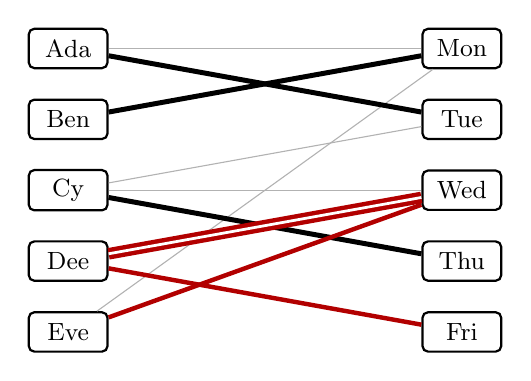
\begin{tikzpicture}[x=50mm, y=9mm, v/.style={draw, thick, rounded corners=2pt, minimum width=10mm, minimum height=5mm,
  font=\small}, n/.style={black!30}, m/.style={line width=1.8pt}, p/.style={line width=1.6pt, red!70!black}]
\foreach \x [count=\i] in {Ada, Ben, Cy, Dee, Eve} { \node[v] (\x) at (0, -\i) {\x}; }
\foreach \x [count=\i] in {Mon, Tue, Wed, Thu, Fri} { \node[v] (\x) at (1, -\i) {\x}; }
\draw[n] (Ada) -- (Mon); \draw[n] (Cy) -- (Tue); \draw[n] (Eve) -- (Mon); \draw[n] (Cy) -- (Wed);
\draw[m] (Ada) -- (Tue); \draw[m] (Ben) -- (Mon); \draw[m] (Cy) -- (Thu);
\draw[p] (Eve) -- (Wed);
\draw[p, double=white, double distance=1pt] (Dee) -- (Wed);
\draw[p] (Dee) -- (Fri);
\end{tikzpicture}
\par\smallskip{\small Before Eve's turn in \cref{out:b2:flows-and-matchings:matching}: the \omterm{def:b2:flows-and-matchings:matching}{matching} is drawn in thick
lines, the other edges in grey. The red augmenting path Eve, Wed, Dee, Fri starts and ends at free vertices; its middle
edge (double line) is in the \omterm{def:b2:flows-and-matchings:matching}{matching}. Exchanging gives Eve--Wed and Dee--Fri, one pair more.}
\end{omfigure}

\begin{theorem}[Berge]\label{thm:b2:flows-and-matchings:berge}
A \omterm{def:b2:flows-and-matchings:matching}{matching} $M$ is maximum if and only if there is no augmenting path relative to $M$.
\end{theorem}

\begin{proof}
If there is an augmenting path $p$, then $M \oplus p$ is a larger \omterm{def:b2:flows-and-matchings:matching}{matching}. Conversely, suppose $M$ is not maximum and
let $M^*$ be a larger \omterm{def:b2:flows-and-matchings:matching}{matching}. In the graph with edges $M \oplus M^*$, every vertex has degree at most $2$, one edge of
each \omterm{def:b2:flows-and-matchings:matching}{matching}; its connected components are therefore paths and cycles whose edges alternate between $M$ and $M^*$. A
cycle that alternates has as many edges of each. Since $|M^*| > |M|$, some path has more edges of $M^*$ than of $M$;
it starts and ends with an edge of $M^*$, and its ends are free in $M$ (an end matched in $M$ would have its $M$-edge
in the component). It is an augmenting path relative to $M$.
\end{proof}

The listing calls the search once from each left vertex, with fresh marks each time. A search visits each edge at most
once, so the whole costs $O(|L| \cdot |E|)$. It is enough to try each left vertex once: a left vertex from which no
augmenting path starts never gets one after later augmentations, a fact we admit (\cref{exo:b2:flows-and-matchings:6}
shows what goes wrong when the marks are shared between searches).

\begin{definition}[Vertex cover]\label{def:b2:flows-and-matchings:vertex-cover}
A \emph{vertex cover}\index{vertex cover} of a graph is a set $C$ of vertices such that every edge has at least one end
in $C$.
\end{definition}

Every \omterm{def:b2:flows-and-matchings:vertex-cover}{vertex cover} has at least as many vertices as any \omterm{def:b2:flows-and-matchings:matching}{matching} has edges, since the edges of a \omterm{def:b2:flows-and-matchings:matching}{matching} have
distinct ends and each needs one in the cover. In bipartite graphs the two numbers meet.

\begin{theorem}[K\H{o}nig]\label{thm:b2:flows-and-matchings:konig}
In a bipartite graph, the largest \omterm{def:b2:flows-and-matchings:matching}{matching} and the smallest \omterm{def:b2:flows-and-matchings:vertex-cover}{vertex cover} have the same size.
\end{theorem}

\begin{proof}
Take the network of \omterm{def:b2:flows-and-matchings:matching}{matchings}, but with capacity $|L| + 1$ on the edges from $L$ to $R$; integral \omterm{def:b2:flows-and-matchings:flow}{flows} are still
\omterm{def:b2:flows-and-matchings:matching}{matchings}, so the maximum \omterm{def:b2:flows-and-matchings:flow}{flow} is the size $\nu$ of a maximum \omterm{def:b2:flows-and-matchings:matching}{matching}. Let $(S, T)$ be a minimum \omterm{def:b2:flows-and-matchings:cut}{cut}; its capacity is
$\nu$, at most $|L|$ (the \omterm{def:b2:flows-and-matchings:cut}{cut} $(\{s\}, V \setminus \{s\})$ has capacity $|L|$), so no edge from $L$ to $R$ goes from $S$
to $T$. Its capacity counts the edges $s \to u$ with $u \in L \cap T$ and $v \to t$ with $v \in R \cap S$, so $\nu = |L \cap T| +
|R \cap S|$. The set $C = (L \cap T) \cup (R \cap S)$ is a \omterm{def:b2:flows-and-matchings:vertex-cover}{vertex cover}: an edge $u, v$ with neither end in $C$ would
have $u \in S$ and $v \in T$, an edge from $L$ to $R$ across the \omterm{def:b2:flows-and-matchings:cut}{cut}. So the smallest \omterm{def:b2:flows-and-matchings:vertex-cover}{vertex cover} has at most $\nu$
vertices, and at least $\nu$ by the remark above.
\end{proof}

\Cref{exo:b2:flows-and-matchings:12} builds the cover from a maximum \omterm{def:b2:flows-and-matchings:matching}{matching} directly, with \omterm{def:b2:flows-and-matchings:alternating}{alternating paths}.

\begin{theorem}[Hall]\label{thm:b2:flows-and-matchings:hall}
A bipartite graph with sides $L$ and $R$ has a \omterm{def:b2:flows-and-matchings:matching}{matching} that matches every vertex of $L$ if and only if every set $A
\subseteq L$ has at least $|A|$ neighbours: $|N(A)| \geq |A|$.
\end{theorem}

\begin{proof}
If such a \omterm{def:b2:flows-and-matchings:matching}{matching} exists, the partners of the vertices of $A$ are $|A|$ distinct neighbours. Conversely, suppose no
\omterm{def:b2:flows-and-matchings:matching}{matching} matches all of $L$. By K\H{o}nig's theorem there is a \omterm{def:b2:flows-and-matchings:vertex-cover}{vertex cover} $C$ with $|C| < |L|$. Let $A = L \setminus
C$. Every edge from a vertex of $A$ must be covered by its other end, so $N(A) \subseteq C \cap R$, and
\[
|N(A)| \leq |C \cap R| = |C| - |C \cap L| < |L| - |C \cap L| = |A|. \qedhere
\]
\end{proof}

Hall's condition is checked set by set, and there are $2^{|L|}$ sets. The \omterm{def:b2:flows-and-matchings:flow}{flow} finds a violating set without trying
them: the readers on the \omterm{def:b2:flows-and-matchings:network}{source} side of a minimum \omterm{def:b2:flows-and-matchings:cut}{cut} (\cref{exo:b2:flows-and-matchings:10}).

\omcode{code/bachelor-2/26-flows-and-matchings/listings/hall.py}{5}{20}{When a sixth reader makes a perfect \omterm{def:b2:flows-and-matchings:matching}{matching}
impossible, the minimum \omterm{def:b2:flows-and-matchings:cut}{cut} names the readers who compete for too few days}\label{lst:b2:flows-and-matchings:hall}

\omoutput{code/bachelor-2/26-flows-and-matchings/outputs/hall.txt}{Three readers available on two days only: Hall's
condition fails for them.}\label{out:b2:flows-and-matchings:hall}

\section{Problems modelled as flows}\label{sec:b2:flows-and-matchings:modelling}

Much of the use of maximum \omterm{def:b2:flows-and-matchings:flow}{flows} is in reductions: a problem that mentions no \omterm{def:b2:flows-and-matchings:flow}{flow} is turned into a network whose
maximum \omterm{def:b2:flows-and-matchings:flow}{flow} or minimum \omterm{def:b2:flows-and-matchings:cut}{cut} is the answer.

\paragraph{Routes with no road in common.}

\begin{definition}[Edge-disjoint paths]\label{def:b2:flows-and-matchings:disjoint}
Paths are \emph{edge-disjoint}\index{edge-disjoint paths} if no edge belongs to two of them. A set of edges
\emph{separates} $t$ from $s$ if every path from $s$ to $t$ uses one of them.
\end{definition}

\begin{theorem}[Menger]\label{thm:b2:flows-and-matchings:menger}
In a directed graph, the largest number of \omterm{def:b2:flows-and-matchings:disjoint}{edge-disjoint paths} from $s$ to $t$ equals the smallest number of edges that
separate $t$ from $s$.
\end{theorem}

\begin{proof}
Give every edge capacity $1$. \omterm{def:b2:flows-and-matchings:disjoint}{Edge-disjoint paths} carry together a \omterm{def:b2:flows-and-matchings:flow}{flow} of \omterm{def:b2:flows-and-matchings:flow}{value} their number, so the largest number of
paths is at most the maximum \omterm{def:b2:flows-and-matchings:flow}{flow}. Conversely, take an integral maximum \omterm{def:b2:flows-and-matchings:flow}{flow}, of \omterm{def:b2:flows-and-matchings:flow}{value} $k$, with values in $\{0, 1\}$.
From $s$, follow edges of \omterm{def:b2:flows-and-matchings:flow}{flow} $1$: conservation lets the walk leave every vertex it enters, until it reaches $t$; if it
comes back to a vertex, drop the loop. Removing the \omterm{def:b2:flows-and-matchings:flow}{flow} on this path gives a \omterm{def:b2:flows-and-matchings:flow}{flow} of \omterm{def:b2:flows-and-matchings:flow}{value} $k - 1$; repeating gives $k$
\omterm{def:b2:flows-and-matchings:disjoint}{edge-disjoint paths}. So the largest number of paths is the maximum \omterm{def:b2:flows-and-matchings:flow}{flow}. A minimum \omterm{def:b2:flows-and-matchings:cut}{cut} has capacity the number of its
edges from $S$ to $T$, and these separate $t$ from $s$; conversely, the vertices still reachable from $s$ after removing
a separating set $F$ form a \omterm{def:b2:flows-and-matchings:cut}{cut} whose edges from $S$ to $T$ are all in $F$. So the smallest separating set is a minimum
\omterm{def:b2:flows-and-matchings:cut}{cut}, and \cref{thm:b2:flows-and-matchings:maxflow-mincut} concludes.
\end{proof}

For roads that can be travelled both ways, each road becomes two opposite edges of capacity $1$; a maximum \omterm{def:b2:flows-and-matchings:flow}{flow} found by
augmentation never uses both, because the second would cancel the first.

\omoutput{code/bachelor-2/26-flows-and-matchings/outputs/disjoint_paths.txt}{Three pairs of places, each joined by three
routes with no road in common.}\label{out:b2:flows-and-matchings:disjoint}

\paragraph{Assignment with capacities.} When the reading room has several seats a day, the edge from a day to the \omterm{def:b2:flows-and-matchings:network}{sink}
gets the number of seats as capacity, and the \omterm{def:b2:flows-and-matchings:flow}{flow} places as many readers as possible; a reader who can come only once a
week keeps an edge of capacity $1$ from the \omterm{def:b2:flows-and-matchings:network}{source} (\cref{exo:b2:flows-and-matchings:9}).

\paragraph{Choosing projects.} The library can run projects that each bring a yearly profit, but each needs equipment
that has to be bought, and the equipment is shared. Which projects should it run? Put an edge from $s$ to each project,
of capacity its profit; an edge from each piece of equipment to $t$, of capacity its cost; and an edge of very large
capacity from each project to each piece of equipment it needs. A \omterm{def:b2:flows-and-matchings:cut}{cut} of finite capacity whose \omterm{def:b2:flows-and-matchings:network}{source} side contains a
project must contain its equipment, else a large edge would cross it. Its capacity is the profits of the projects
left out plus the costs of the equipment bought, which is the total of all profits minus the net profit of the
projects run. A minimum \omterm{def:b2:flows-and-matchings:cut}{cut} gives the best choice.

\omoutput{code/bachelor-2/26-flows-and-matchings/outputs/selection.txt}{The library's projects chosen by a minimum \omterm{def:b2:flows-and-matchings:cut}{cut},
checked against the 32 choices.}\label{out:b2:flows-and-matchings:selection}

\begin{history}
% ledger: b2:menger-1927
% ledger: b2:konig-1931
% ledger: b2:hall-1935
The combinatorial theorems came first. Karl Menger published his theorem on disjoint paths in 1927, in a paper on the
theory of curves; D\'enes K\H{o}nig proved his theorem on bipartite graphs in 1931, and Jen\H{o} Egerv\'ary
independently the same year in a more general form with weights; Philip Hall published his condition in 1935. The
\omterm{def:b2:flows-and-matchings:flow}{max-flow} \omterm{def:b2:flows-and-matchings:cut}{min-cut} theorem of 1956 contains them all.
\end{history}

\section{Exercises}\label{sec:b2:flows-and-matchings:exercises}

\begin{exercise}[$\star$]\label{exo:b2:flows-and-matchings:1}
On the network of \cref{out:b2:flows-and-matchings:flow}, which of the following are \omterm{def:b2:flows-and-matchings:flow}{flows}, and of which \omterm{def:b2:flows-and-matchings:flow}{value}?
$f_1$: $sa\,7$, $sb\,5$, $ac\,5$, $ad\,2$, $bc\,5$, $ct\,7$, $dt\,2$; $f_2$: $sa\,8$, $sb\,6$, $ac\,3$, $ad\,5$, $bc\,6$,
$ct\,9$, $dt\,5$; $f_3$: $sa\,6$, $sb\,6$, $ac\,1$, $ad\,5$, $bc\,6$, $ct\,7$, $dt\,5$. Check with \code{exo_is_flow.py}.
\end{exercise}

\begin{exercise}[$\star$]\label{exo:b2:flows-and-matchings:2}
In \code{exo_no_reverse.py}, a network whose \omterm{def:b2:flows-and-matchings:residual}{residual capacity} is only the unused capacity of each edge is given to the
same algorithm. What \omterm{def:b2:flows-and-matchings:flow}{value} does it find on the network of \cref{out:b2:flows-and-matchings:flow}, and why? Which line of
\cref{lst:b2:flows-and-matchings:network} does it miss?
\end{exercise}

\begin{exercise}[$\star$]\label{exo:b2:flows-and-matchings:3}
Find a maximum \omterm{def:b2:flows-and-matchings:flow}{flow} and a minimum \omterm{def:b2:flows-and-matchings:cut}{cut} by hand for the network with edges $s \to x$ (9), $s \to y$ (7), $x \to y$ (3),
$x \to z$ (4), $y \to w$ (6), $z \to y$ (2), $z \to t$ (5), $w \to t$ (7). Then check with \code{exo_maxflow.py}.
\end{exercise}

\begin{exercise}[$\star$]\label{exo:b2:flows-and-matchings:4}
In the bad example, show that the augmenting paths $s, a, b, t$ and $s, b, a, t$, taken alternately, take exactly $2C$
augmentations, and that breadth-first search takes $2$. Compare with \cref{out:b2:flows-and-matchings:bad}.
\end{exercise}

\begin{exercise}[$\star\star$]\label{exo:b2:flows-and-matchings:5}
Take the \omterm{def:b2:flows-and-matchings:flow}{flow} $f_3$ of \cref{exo:b2:flows-and-matchings:1}. Compute its \omterm{def:b2:flows-and-matchings:residual}{residual network}, the vertices reachable from
$s$, and deduce without any further computation that $f_3$ is maximum. Check with \code{exo_mincut.py}.
\end{exercise}

\begin{exercise}[$\star\star$]\label{exo:b2:flows-and-matchings:6}
In \code{exo_match_bug.py}, the marks of the search are created once for all the left vertices instead of once per
vertex. On the readers of \cref{out:b2:flows-and-matchings:matching} it matches 3 instead of 5. Follow the run and
explain which augmenting path it misses.
\end{exercise}

\begin{exercise}[$\star\star$]\label{exo:b2:flows-and-matchings:7}
In \cref{out:b2:flows-and-matchings:disjoint}, find for each pair three roads that separate the two places. Then change
the network so that the routes share no place either (other than their ends): split each place into an entrance and an
exit joined by an edge of capacity $1$. Compare the numbers given by \code{exo_vertex_disjoint.py}.
\end{exercise}

\begin{exercise}[$\star\star$]\label{exo:b2:flows-and-matchings:8}
Prove \cref{prop:b2:flows-and-matchings:flow-across-cut}.
\end{exercise}

\begin{exercise}[$\star\star$]\label{exo:b2:flows-and-matchings:9}
Forty readers share a reading room open on 8 slots; reader $k$, for $k = 1$ to $40$, can come at the slots $k \bmod 8$, $3k \bmod 8$ and
$(5k + 1) \bmod 8$, once a week. Model the assignment as a \omterm{def:b2:flows-and-matchings:flow}{flow}. Run \code{exo_readers.py} with 5 seats per slot, then with
the seats $2, 2, 5, 5, 6, 6, 7, 7$, and explain why 40 seats do not place 40 readers.
\end{exercise}

\begin{exercise}[$\star\star\star$]\label{exo:b2:flows-and-matchings:10}
Prove Hall's theorem directly from the \omterm{def:b2:flows-and-matchings:flow}{max-flow} \omterm{def:b2:flows-and-matchings:cut}{min-cut} theorem, with the network of \cref{lst:b2:flows-and-matchings:hall}:
if the maximum \omterm{def:b2:flows-and-matchings:flow}{flow} is below $|L|$, show that the vertices of $L$ on the \omterm{def:b2:flows-and-matchings:network}{source} side of a minimum \omterm{def:b2:flows-and-matchings:cut}{cut} form a set $A$ with
$|N(A)| < |A|$.
\end{exercise}

\begin{exercise}[$\star\star\star$]\label{exo:b2:flows-and-matchings:11}
Prove \cref{lem:b2:flows-and-matchings:monotone}. Suppose some distance decreases, choose $v$ of smallest new distance
among the vertices whose distance decreased, and look at the last edge $(u, v)$ of a shortest path to $v$ in $G_{f'}$.
\end{exercise}

\begin{exercise}[$\star\star\star$]\label{exo:b2:flows-and-matchings:12}
Let $M$ be a maximum \omterm{def:b2:flows-and-matchings:matching}{matching} of a bipartite graph, and $Z$ the set of vertices reachable from the free vertices of $L$
by \omterm{def:b2:flows-and-matchings:alternating}{alternating paths} (starting with an edge out of $M$). Prove that $(L \setminus Z) \cup (R \cap Z)$ is a \omterm{def:b2:flows-and-matchings:vertex-cover}{vertex cover}
of size $|M|$. Implement it, and check it on the readers of \cref{out:b2:flows-and-matchings:hall} against all subsets.
\end{exercise}

\section{Problem: The stadium bus plan}\label{sec:b2:flows-and-matchings:problem}

\begin{problem}[{Weekend problem --- The stadium bus plan}]\label{pb:b2:flows-and-matchings:1}
The town plans the buses from the Bus Depot to the Football Ground for a match, with the network of
\cref{lst:b2:flows-and-matchings:town}. The program below repeats the computation, tries widening each road of the
minimum \omterm{def:b2:flows-and-matchings:cut}{cut}, and assigns drivers to the nine buses.

\omcode{code/bachelor-2/26-flows-and-matchings/listings/bus_plan.py}{10}{32}{The bus plan: the \omterm{def:b2:flows-and-matchings:flow}{flow}, the \omterm{def:b2:flows-and-matchings:cut}{cut}, what
widening each road of the \omterm{def:b2:flows-and-matchings:cut}{cut} buys, and the \omterm{def:b2:flows-and-matchings:cut}{cut} nearest the ground}\label{lst:b2:flows-and-matchings:bus-plan}

\omoutput{code/bachelor-2/26-flows-and-matchings/outputs/bus_plan.txt}{120 buses an hour, two minimum \omterm{def:b2:flows-and-matchings:cut}{cuts}, and the
drivers.}\label{out:b2:flows-and-matchings:problem}

\needspace{4\baselineskip}\medskip\noindent\textbf{Part I --- The model.}\par\nopagebreak
\begin{enumerate}
\item The town has 30 places and its roads give 105 directed edges. How many roads are one-way, if the table has 53
roads?
\item The rule gives 20, 40 or 60 buses an hour. Which speeds give these, and is 60 used on the routes of
\cref{out:b2:flows-and-matchings:town}?
\item Why does a two-way road become two edges of the same capacity, rather than one edge whose capacity is shared by both
directions? What would the shared version require?
\item Buses go to the ground and none come back during the hour. Show that a \omterm{def:b2:flows-and-matchings:flow}{flow} from the depot to the ground can be
chosen with no road used in both directions.
\item The ground has a car park for 100 buses an hour. Add it to the model.
\item What does the \omterm{def:b2:flows-and-matchings:flow}{value of a flow} count, in buses, and what does conservation say at the Town Square?
\end{enumerate}

\needspace{4\baselineskip}\medskip\noindent\textbf{Part II --- Augmenting paths.}\par\nopagebreak
\begin{enumerate}[resume, beginpenalty=10000]
\item The first two paths of \cref{out:b2:flows-and-matchings:town} have 2 roads each. Why must breadth-first search
find them first?
\item The third path, 16-4-7-23-10-2-11-6-20-15, goes through the North School and then the Swimming Pool. Which edges
were full at that point, and why can it not end with 4-15 or 7-15?
\item Check that the path lengths are non-decreasing, and say which result guarantees it.
\item Bound the number of augmentations by \cref{thm:b2:flows-and-matchings:edmonds-karp-bound} and by
\cref{thm:b2:flows-and-matchings:integrality}. Which bound is better here?
\item Would a depth-first search for augmenting paths reach 120 too? In how many augmentations at most?
\item Give the \omterm{def:b2:flows-and-matchings:flow}{flow} at the end on road 11, North School > Football Ground, and on road 20, Swimming Pool >
Football Ground, and explain. (Roads are numbered apart from places: the paths print places, the \omterm{def:b2:flows-and-matchings:cut}{cuts} print roads.)
\end{enumerate}

\needspace{4\baselineskip}\medskip\noindent\textbf{Part III --- The bottleneck roads.}\par\nopagebreak
\begin{enumerate}[resume, beginpenalty=10000]
\item Check that the four roads of the first \omterm{def:b2:flows-and-matchings:cut}{cut} carry 120 buses an hour between them, and that every route from the
depot to the ground uses one of them.
\item Widening road 16, Hill Park > Market Hall, by 20 changes nothing. Why is that not a contradiction with the fact that it belongs to a minimum
\omterm{def:b2:flows-and-matchings:cut}{cut}?
\item The program computes a second minimum \omterm{def:b2:flows-and-matchings:cut}{cut}, the one nearest the ground. Describe in words how it is computed, and
check that its capacity is 120.
\item Prove that a road whose widening raises the maximum \omterm{def:b2:flows-and-matchings:flow}{flow} lies in every minimum \omterm{def:b2:flows-and-matchings:cut}{cut}, and check it for roads 11 and 20.
\item Is the converse true: does widening a road that lies in every minimum \omterm{def:b2:flows-and-matchings:cut}{cut} always raise the maximum \omterm{def:b2:flows-and-matchings:flow}{flow}?
\item State the problem's result: max \omterm{def:b2:flows-and-matchings:flow}{flow} = min \omterm{def:b2:flows-and-matchings:cut}{cut} = 120 buses an hour, and the roads in both \omterm{def:b2:flows-and-matchings:cut}{cuts}, 11 and 20, are the
ones to widen. Widening road 20 by 40 instead of 20 still gives 140 buses an hour: which \omterm{def:b2:flows-and-matchings:cut}{cut} limits the \omterm{def:b2:flows-and-matchings:flow}{flow} then?
\end{enumerate}

\needspace{4\baselineskip}\medskip\noindent\textbf{Part IV --- Drivers and buses.}\par\nopagebreak
\begin{enumerate}[resume, beginpenalty=10000]
\item Bus $B_i$ is single-deck, double-deck or electric according to $i \bmod 3$. List the buses of each kind and the
drivers licensed for each.
\item Draw the bipartite graph of drivers and buses, and check the \omterm{def:b2:flows-and-matchings:matching}{matching} printed.
\item When Hal is ill, only 8 buses get a driver. Find a set of buses that violates Hall's condition, on the side of the
buses.
\item Find a \omterm{def:b2:flows-and-matchings:vertex-cover}{vertex cover} of size 8 of the graph without Hal.
\item Which single driver, added with one licence, would restore 9 buses? Is there more than one answer?
\item Each driver can make two trips in the afternoon and each bus three. Model the assignment of trips as a \omterm{def:b2:flows-and-matchings:flow}{flow}.
\end{enumerate}
\end{problem}
